\documentclass[12pt,a4paper,titlepage]{scrartcl}

\usepackage[main=ngerman,english]{babel}
\usepackage[utf8]{inputenc}
\usepackage[T1]{fontenc}
\usepackage{lmodern}
\usepackage{geometry}
\geometry{left=2.5cm,right=2.5cm,top=2.5cm,bottom=3cm,head=29pt,foot=25pt}
\setlength{\footheight}{25pt}
\usepackage{microtype}
\usepackage{amsmath,amssymb,mathtools}
\numberwithin{equation}{section}
\usepackage{siunitx}
\sisetup{locale=DE, separate-uncertainty=true, per-mode=fraction}
\usepackage{booktabs}
\usepackage{multirow}
\usepackage{graphicx}
\usepackage{float}
\usepackage{caption}
\usepackage{subcaption}
\usepackage[automark]{scrlayer-scrpage}
\usepackage[most]{tcolorbox}
\usepackage{hyperref}
\usepackage{pdfpages}
\usepackage{csvsimple-l3}
\usepackage{longtable}
\usepackage{graphicx}


\hypersetup{colorlinks=true, linkcolor=blue!60!black, urlcolor=blue!60!black, citecolor=blue!60!black}

\clearpairofpagestyles

\chead{%
    \versuch\hfill\autor\
    \rule{\textwidth}{0.2pt}%
}
\cfoot{%
    \rule{\textwidth}{0.2pt}\\[-0.5ex]
    \pagemark\
}
\addtokomafont{pagefoot}{\small}

\newtcolorbox{resultbox}[1][]{ 
    enhanced,
    colback=black!4!white,
    colframe=black!65!black,
    boxrule=0.8pt,
    arc=0.0mm,
    title=#1,
    fonttitle=\bfseries,
    %drop shadow
}


\newcommand{\versuch}{Versuch 22}
\newcommand{\titel}{Titel des Versuchs}
\newcommand{\praktikum}{Physikalisches Anfängerpraktikum 1}
\newcommand{\autor}{Jonathan Gießen}
\newcommand{\gruppe}{Gruppe 8}
\newcommand{\datum}{31. August 2026}
\newcommand{\betreuer}{Tutor/in}

\begin{document}

\pagestyle{scrheadings}

\begin{titlepage}
    \centering
    {\Large \praktikum\par}
    \vspace{0.8cm}
    {\LARGE \bfseries \versuch\ -- \titel\par}
    \vspace{1.5cm}

    \begin{tabular}{ll}
        \textbf{Autor:} & \autor\\
        \textbf{Gruppe:} & \gruppe\\
        \textbf{Betreuer:} & \betreuer\\
        \textbf{Datum:} & \datum\\
    \end{tabular}

    \vfill
    \hrulefill\
\end{titlepage}

\tableofcontents
\newpage

\section{Einleitung}
\subsection{Motivation}

In diesem Versuch wird die Elementarladung Nach Millikan bestimmt. Dazu wird die Bewegung von Öltröpfchen
in einem elektrischen Feld untersucht. 
Ziel ist es, die Ladung der Tröpfchen zu messen und daraus die Elementarladung zu bestimmen.
Den Physikern Robert Millikan und Harvey Fletcher gelang es 1910, die Elementarladung genauer,
als ihre Vorgänger, zu bestimmen. 
\newline 
1923 erhielt Millikan dafür den Nobelpreis für Physik.

\section{Grundlagen und Theorie}

\subsection{Auf die Öltröpfchen wirkende Kräfte}

Der Versuch basiert auf der Tatsache, dass die Bewegung von Öltröpfchen in einem elektrischen Feld durch die Coulomb-Kraft beeinflusst wird. 
Die Tröpfchen werden durch die Gravitation nach unten gezogen, während das elektrische Feld eine Kraft in entgegengesetzter Richtung ausübt. 
Durch die Messung der Geschwindigkeit der Tröpfchen unter verschiedenen Bedingungen kann die Ladung der Tröpfchen bestimmt werden.
Das annähern homogene elektrische Feld wird durch einen Plattenkondensator erzeugt, dessen Plattenabstand bekannt ist.
\newline 
Gemessen wird die Fallgeschiwindigkeit $v_f$ eines Tröpfchens, wenn das elektrische Feld ausgeschaltet ist,
und die Steiggeschwindigkeit $v_s$, wenn das elektrische Feld eingeschaltet ist.
Kleine Flüssigkeitströpfchen sind im Allgemeinen geladen. Ihre Ladung ist notwendigerweise ein ganzzahliges Vielfaches der
Elementarladung. Betrachtet man ein in Luft befindliches geladenes Tröpfchen in einem vertikal
gerichteten elektrischen Feld E, wirken die Beträge der folgenden Kräfte:

\begin{align}
    F_g &= \frac{4}{3}\pi r^3 \rho_{\text{Öl}} g
    && \text{(Gewichtskraft)} \label{Gravitation} \\[0.5em]
    F_a &= \frac{4}{3}\pi r^3 \rho_{\text{Luft}} g
    && \text{(Auftriebskraft)} \label{Auftrieb} \\[0.5em]
    F_e &= qE = q\frac{U}{d}
    && \text{(Coulombkraft)} \label{Coulombkraft} \\[0.5em]
    F_R &= 6\pi\eta r v
    && \text{(Stokesche Reibungskraft)} \label{Stokes}
\end{align}

\begin{figure}[htbp]
  \centering
  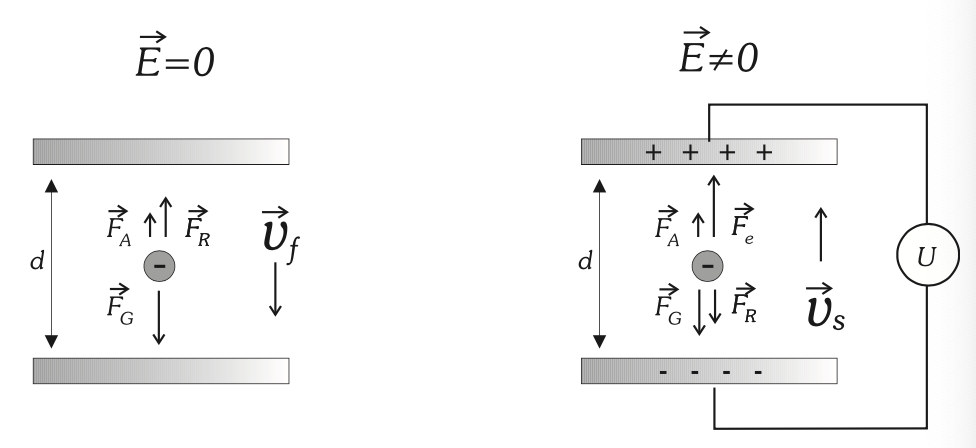
\includegraphics[width=0.8\textwidth]{Froces_millikan.png} 
  \caption{Kräfte auf ein Öltröpfchen in einem elektrischen Feld.} 
    \label{Kräfteol}
\end{figure}


\medskip

\noindent
Wobei $r$ der Radius des Tröpfchens, $\rho_{\text{Öl}}$ die Dichte des Öls, $\rho_{\text{Luft}}$ die Dichte der Luft, $g$ die Erdbeschleunigung,
$q$ die Ladung des Tröpfchens, $E$ die elektrische Feldstärke, $U$ die angelegte Spannung, $d$ der Plattenabstand und $\eta$ die Viskosität der Luft ist.



\subsection{Sinkbewegung ohne elektrisches Feld}
Beim antriebslosen Sinken mit konstanter Sinkgeschwindigkeit $v_{\text{f}}$ 
(Kräftegleichgewicht zwischen Reibungskraft und Gewichtskraft und Auftriebskraft) gilt mit 
$\rho = \rho_{\text{Öl}} - \rho_{\text{Luft}}$:
\begin{equation}
    F_{\text{R,fall }} = F_{\text{G}} - F_{\text{A}} \implies 6\pi\eta r v_{\text{f}} = \frac{4}{3}\pi r^3 \rho g
\end{equation}
Auflösen nach dem Tröpfchenradius $r$:
\begin{equation}
    r^2 = \frac{9\eta v_{\text{f}}}{2\rho g} \implies r = \sqrt{\frac{9\eta}{2\rho g}v_{\text{f}}} \label{radius}
\end{equation}

\noindent
\subsection{Steigbewegung im elektrischen Feld}

Wird ein elektrisches Feld so angelegt, dass das geladene Tröpfchen mit konstanter Steiggeschwindigkeit $v_{\text{s}}$ nach oben steigt, wirkt die elektrische Kraft nach oben, während Reibungskraft und Gewichtskraft nach unten wirken:
\begin{equation}
    F_{\text{el}} = F_{\text{G}} + F_{\text{R,s}}
\end{equation}
Einsetzen der Kräfte $F_{\text{el}} = q \frac{U}{d}$, $F_{\text{R,s}} = 6\pi\eta r v_{\text{s}}$ sowie $F_{\text{G}} = F_{\text{R,fall}} = 6\pi\eta r v_{\text{f}}$ liefert:
\begin{align}
    q \frac{U}{d} &= 6\pi\eta r v_{\text{f}} + 6\pi\eta r v_{\text{s}} \\
    q \frac{U}{d} &= 6\pi\eta r (v_{\text{f}} + v_{\text{s}})
\end{align}
Auflösen nach der Ladung $q$:
\begin{equation}
    q = (v_{\text{f}} + v_{\text{s}}) \cdot \frac{6\pi\eta r d}{U}
\end{equation}
Setzt man den Radius $r = \sqrt{\frac{9\eta v_{\text{f}}}{2\rho g}}$ in den Ausdruck für $q$ ein, erhält man:
\begin{equation}
    q = (v_{\text{f}} + v_{\text{s}}) \frac{6\pi d}{U} \sqrt{\frac{9 v_{\text{f}} \eta^3}{2\rho g}} \label{Ladung}
\end{equation}
\subsection{Cunningham-Korrektur}

Die zuvor berechneten Ladungen der Öltröpfchen weisen gegenüber der
Elementarladung eine systematische Abweichung auf. Der bestimmte Wert ist
dabei typischerweise um etwa den Faktor $1{,}1$ zu groß. Diese Abweichung
nimmt für kleinere Tröpfchenradien weiter zu.
\newline
Die Ursache liegt darin, dass die Radien der Öltröpfchen ungefähr im Bereich
von $\SIrange{e-6}{e-7}{\meter}$ liegen und damit eine ähnliche Größenordnung
wie die mittlere freie Weglänge der Luftmoleküle (\SI{6.8e-8}{\meter}) besitzen. 
Für eine sehr genaue Bestimmung ist die Annahme einer konstanten Luftviskosität unter diesen Bedingungen nicht mehr ausreichend.
Sie gilt nur, wenn der Durchmesser der Tröpfchen deutlich größer als die
mittlere freie Weglänge der Luftmoleküle ist.
\newline
Daher wird die Viskosität durch einen radiusabhängigen Korrekturfaktor
angepasst. Die Cunningham-Korrektur des Stokes'schen Gesetzes lautet:
\begin{equation}
    \eta(r) = \eta_0 f(r)
    = \eta_0\left(1+\frac{B}{pr}\right),
    \label{Cunningham}
\end{equation}
wobei $\eta_0$ die nichtkorrigierte Viskosität, $r$ der Tröpfchenradius,
$p$ der Luftdruck und $B$ eine empirische Konstante ist.\newline
Da der Tröpfchenradius $r$ selbst von $\eta(r)$ abhängt,
würde ein exaktes Einsetzen in die Gleichung für den Radius zu einer quadratischen Gleichung führen.
Für die praktische Auswertung genügt es jedoch, den Radius $r$ zunächst näherungsweise mit $\eta_0$ zu bestimmen:
\begin{equation}
    r \approx \sqrt{\frac{9\eta_0 v_{\text{f}}}{2\rho g}}
\end{equation}
Der dadurch bei der Berechnung von $r$ entstehende Fehler von etwa 5\,\% pflanzt sich im Korrekturfaktor $f(r)$ lediglich als Abweichung von circa 0,5\,\% fort,
was im Rahmen der Messgenauigkeit vernachlässigbar ist.
Somit bleibt Gleichung\,\eqref{Ladung} vorerst gültig, wobei $\eta$ durch die korrigierte Viskosität $\eta(r)$ ersetzt wird.
Einsetzen der korrigierten Viskosität $\eta(r)$ in die Gleichung für die Ladung $q$ liefert:
\begin{equation}
    q = (v_{\text{f}} + v_{\text{s}}) \frac{6\pi d}{U} \sqrt{\frac{9 v_{\text{f}} (\eta_\text{0}f(r))^3}{2\rho g}} \label{Ladung_korrigiert}
\end{equation}

\subsection{Literaturwerte}

Für die Auswertung werden folgende Konstanten und Geräteparameter verwendet:

\begin{table}[H]
    \centering
    \caption{Für die Auswertung verwendete Konstanten und Geräteparameter.}
    \begin{tabular}{ll}
        \toprule
        Größe & Wert \\
        \midrule
        Viskosität der Luft & $\eta_0 = \SI{1.81e-5}{\newton\second\per\meter\squared}$ \\
        Schwerebeschleunigung & $g = \SI{9.81}{\meter\per\second\squared}$ \\
        Dichte des Öls bei \SI{15}{\celsius} & $\rho_{\text{Öl}} = \SI{877}{\kilogram\per\meter\cubed}$ \\
        Dichte des Öls bei \SI{25}{\celsius} & $\rho_{\text{Öl}} = \SI{871}{\kilogram\per\meter\cubed}$ \\
        Dichte der Luft & $\rho_{\text{Luft}} = \SI{1.29}{\kilogram\per\meter\cubed}$ \\
        Konstante im Korrekturfaktor & $b = \SI{7.78e-3}{\pascal\meter}$ \\
        Abstand der Kondensatorplatten & $d = \SI{6.00 +- 0.05}{\milli\meter}$ \\
        Skala auf dem Bildschirm & $1\,\mathrm{Skt} = \SI{5.00 +- 0.13 e-5}{\meter}$ \\
        \bottomrule
    \end{tabular}
\end{table}





\section{Messprotokoll}

\subsection{Versuchsaufbau und Aufgaben}
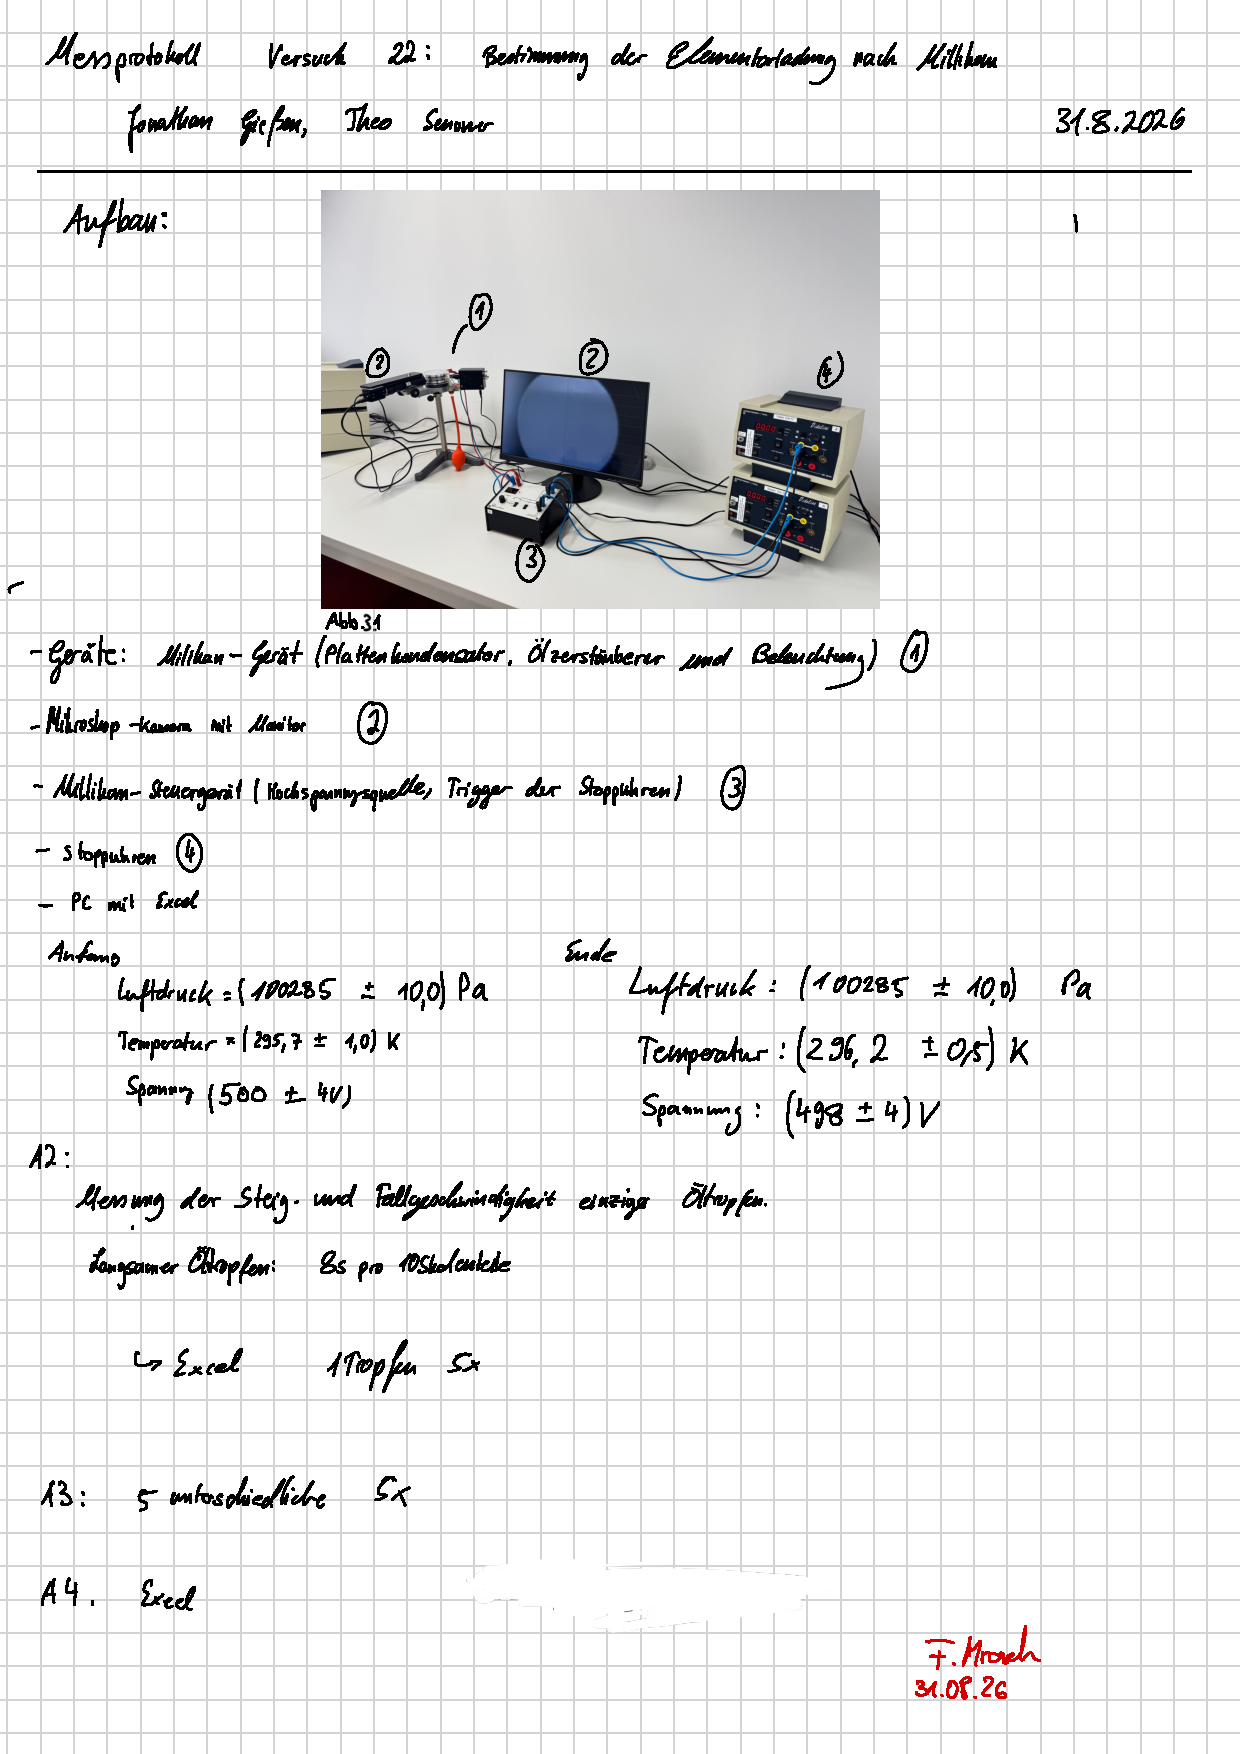
\includepdf[
    pages=-,
    width=\textwidth,
    height=\textheight,
    keepaspectratio,
    pagecommand={\thispagestyle{scrheadings}}
]{../Messprotokoll 22.pdf}

\subsection{Durchführung}

Zu Beginn des Versuchs wurden der barometrische Luftdruck ${p = 100285 \pm 10\,\text{Pa}}$ sowie
die Raumtemperatur zu Versuchsbeginn ($T = 295{,}7\pm 1{,}0\,\text{K} \approx 22{,}5\,^\circ\text{C}$) und zum
Versuchsende ($T = 296{,}2\pm 1{,}0\,\text{K}$) notiert. Am Plattenkondensator wurde eine Spannung von ca.~$500\,\text{V}$ (gemessen: $(500 \pm 4)\,\text{V}$) 
eingestellt und für die gesamte Messdauer konstant gehalten.
Über den Ölzerstäuber wurden Tröpfchen in den Kondensatorraum eingebracht und mit dem Mikroskop über den Monitor fokussiert. Die Streckenmessung erfolgte
anhand der auf dem Monitor eingeblendeten Skala ($1\,\text{Skt} = (5{,}00 \pm 0{,}13)\cdot 10^{-5}\,\text{m}$).
Für die Messungen wurden bevorzugt langsam steigende Tröpfchen ausgewählt.

\medskip
Für die Auswertung wurden folgende Messungen durchgeführt:
\begin{itemize}
    \item \textbf{Mehrfachmessung an einem Tröpfchen (Aufgabe 2):} An einem einzelnen Öltröpfchen wurden die Fallzeit $t_1$ (im feldfreien Raum, $E=0$) sowie die Steigzeit $t_2$ (mit angelegtem elektrischem Feld, $E \neq 0$) jeweils fünfmal hintereinander über eine definierte Strecke (z.\,B.~$10\,\text{Skt}$) gemessen, um die statistische Streuung der Geschwindigkeitsmessung abzuschätzen.
    \item \textbf{Messreihe an verschiedenen Tröpfchen (Aufgaben 3 \& 4):} Insgesamt wurden 30 Wertepaare (bestehend aus je einer Fall- und einer Steigzeit, also 60 Einzelzeitmessungen)
    an unterschiedlichen Öltröpfchen aufgenommen. Dabei wurden sowhol schnellere, als auch lagsamere Tröpfchen berücksichtigt, um eine möglichst große Bandbreite an Tröpfchengeschwindigkeiten zu erfassen.
    Bei fünf Tröpfchen wurden jeweils fünf Zyklen durchlaufen. 
\end{itemize}
Für jedes Tröpfchen wurden Fallweg, Fallzeit, Steigweg und Steigzeit zusammen mit den Umgebungsparametern und der Kondensatorspannung in das vorbereitete Auswerteblatt eingetragen, um über die Cunningham-korrigierten Viskositäten die Tröpfchenradien und Ladungen zu berechnen.

\subsection{Messwerte}
Für die Bestimmung der Elementarladung werden in einer Exceltabelle die Messwerte eingetragen und die Ladung der Tröpfchen berechnet.
\begin{figure}[htbp]
    \centering
    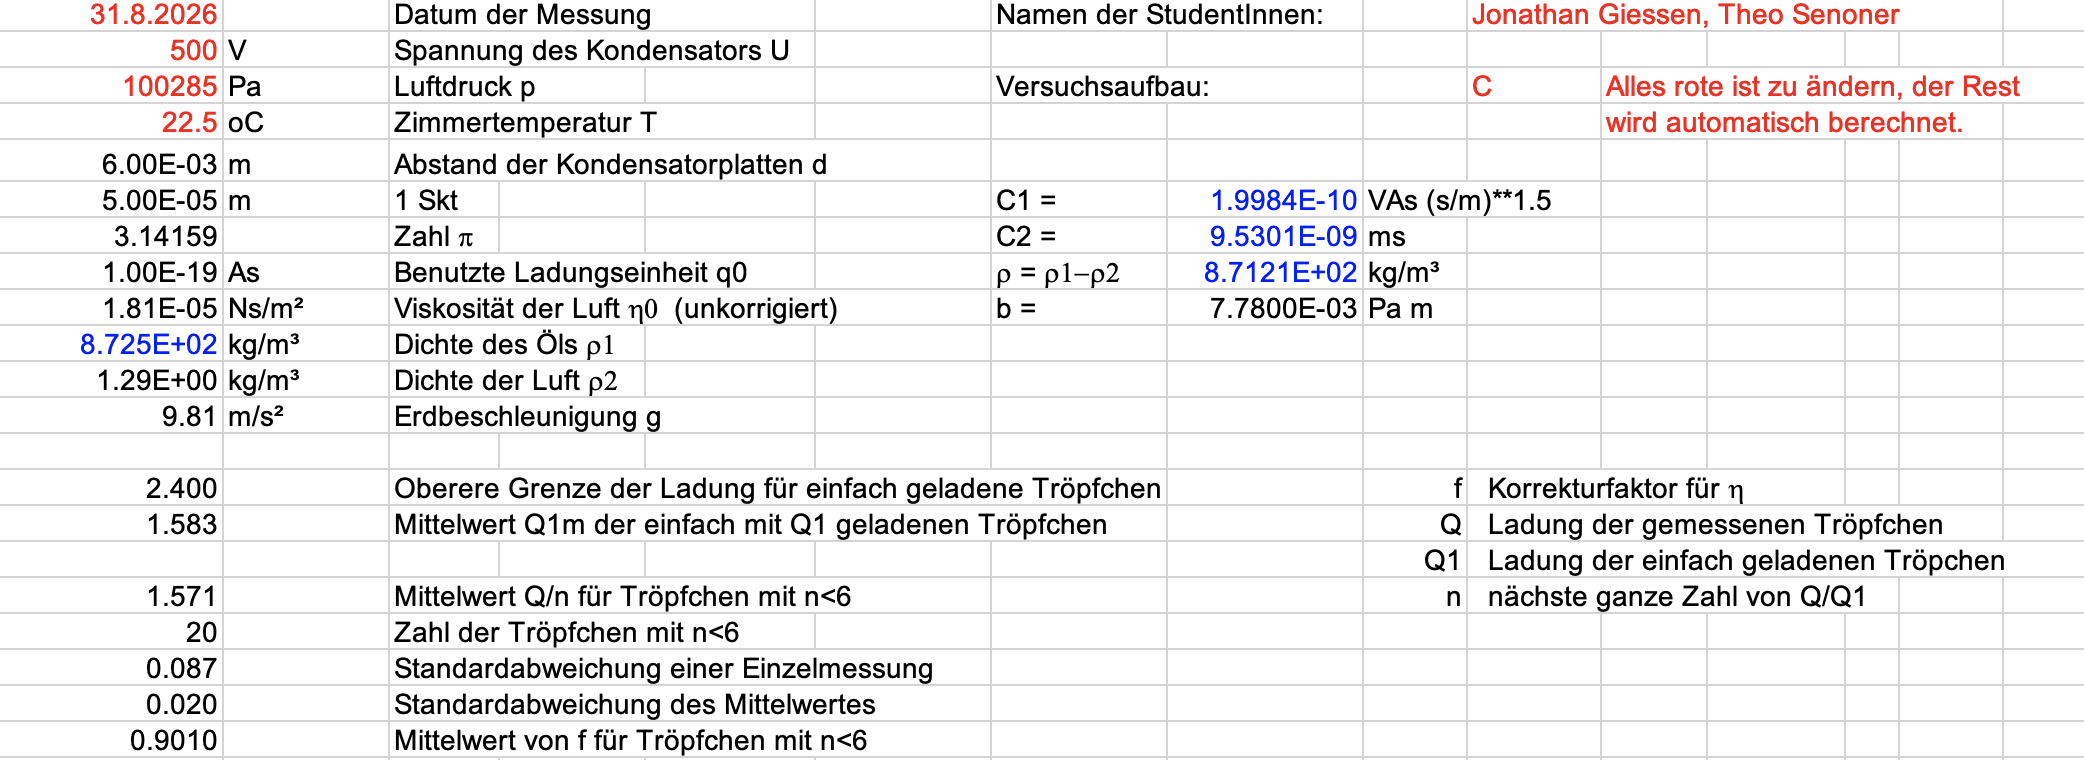
\includegraphics[width=0.8\textwidth]{Hilfsvariable.png} 
    \caption{Hilfsvariablen.} 
    \label{Helpvariable}

\end{figure}

\begin{table}[htbp]
  \centering
  \small
  \caption{Messwerte zur Bestimmung der Elementarladung.}
    \resizebox{\textwidth}{!}{%
        \csvautotabular{../Versuch22_Values.csv}%
    }
\end{table}









\section{Auswertung}

Die Messwerte wurden zunächst grafisch dargestellt und anschließend mit einer linearen Ausgleichsrechnung analysiert. Die Gerade hat die Form
\begin{equation}
    y = a x + b.
\end{equation}

Aus der linearen Regression folgt:
\begin{equation}
    a = \frac{\sum (x_i-\bar{x})(y_i-\bar{y})}{\sum (x_i-\bar{x})^2},
    \qquad
    b = \bar{y} - a\bar{x}.
\end{equation}
\begin{resultbox}[67 ergbenis]
    Die experimentell bestimmte Steigung beträgt
    \[
        a = \SI{2.14}{\second\per\meter}
    \]
    und der Achsenabschnitt ist
    \[
        b = \SI{0.02}{\second}.
    \]
\end{resultbox}

\subsection{Fehlerrechnung}

Die Messunsicherheit wurde mit der Standardabweichung des Mittelwerts bestimmt:
\begin{equation}
    u_{\bar{x}} = \frac{s}{\sqrt{N}}.
\end{equation}

Die relative Abweichung zum erwarteten Wert $y_{\mathrm{theor}}$ ergibt sich aus
\begin{equation}
    \Delta = \frac{|y_{\mathrm{exp}} - y_{\mathrm{theor}}|}{y_{\mathrm{theor}}}\times 100\,\%.
\end{equation}

\subsection{Grafische Darstellung}

\begin{figure}[H]
    \centering
    \includegraphics[width=0.8\textwidth]{example-image}
    \caption{Beispielhafte Darstellung der Messdaten mit Ausgleichsgerade.}
\end{figure}

\section{Diskussion}

Die Ergebnisse zeigen eine gute Übereinstimmung mit dem theoretischen Modell. Die geringe Abweichung von \dots spricht für eine zufriedenstellende Messgenauigkeit. Mögliche Ursachen für systematische Abweichungen sind \dots.

Die Messwerte sind insgesamt konsistent, jedoch sind mögliche Fehlerquellen wie \dots, \dots und \dots zu berücksichtigen. Eine Verfeinerung der Messmethode könnte die Genauigkeit weiter erhöhen.

\section{Fazit}

Der Versuch zeigt, dass \dots dem erwarteten physikalischen Zusammenhang folgt. Die gemessenen Werte bestätigen die Theorie innerhalb der Messunsicherheit. Die gewonnenen Ergebnisse sind für die grundlegende experimentelle Analyse des Praktikums geeignet.

\appendix
\section{Anhang}

Weitere Messdaten, Berechnungen oder Rohdaten können hier ergänzt werden.

\end{document}
